\documentclass[tikz,border=3.14mm]{standalone}
\usepackage{pgfplots}
\pgfplotsset{compat=1.18}

\begin{document}
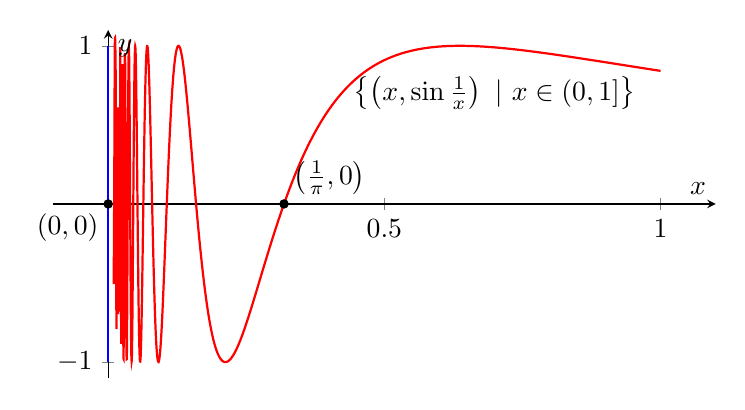
\begin{tikzpicture}
    \begin{axis}[
        width=10cm,
        height=6cm,
        xmin=-0.1, xmax=1.1,
        ymin=-1.1, ymax=1.1,
        axis lines=middle,
        xlabel={$x$},
        ylabel={$y$},
        xtick={0,0.5,1},
        ytick={-1,0,1},
        samples=1000,
        clip=false
    ]
    
    % Вертикальный отрезок в нуле
    \draw[thick, blue] (0,-1) -- (0,1);
    
    % Синусоидальная часть (x ∈ (0,1])
    \addplot[domain=0.01:1, smooth, thick, red] {sin(deg(1/x))};
    
    % Подписи
    %\node at (0.2,0.5) {$\{(0,y)\ |\ y\in[-1,1]\}$};
    \node at (0.7,0.7) {$\left\{\left(x,\sin\frac{1}{x}\right)\ |\ x\in(0,1]\right\}$};
    
    % Примеры точек
    \filldraw (0,0) circle (1.5pt) node[below left] {$(0,0)$};
    \filldraw (1/pi,0) circle (1.5pt) node[above right] {$\left(\frac{1}{\pi},0\right)$};
    
    \end{axis}
\end{tikzpicture}
\end{document}